%%% Template originaly created by Karol Kozioł (mail@karol-koziol.net) and modified for ShareLaTeX use

\documentclass[letterpaper,10pt]{article}
\usepackage[letterpaper]{geometry}
\usepackage{url}
\usepackage[T1]{fontenc}
\usepackage[utf8]{inputenc}
\usepackage{graphicx}
\usepackage{xcolor}
\usepackage{url}
\renewcommand\familydefault{\sfdefault}
\usepackage{tgheros}
\usepackage[defaultmono]{droidmono}

\usepackage{amsmath,amssymb,amsthm,textcomp}
\usepackage{enumerate}
\usepackage{multicol}
\usepackage{tikz}
\usepackage{float}

\DeclareMathOperator*{\argmin}{argmin}
\DeclareMathOperator*{\argmax}{argmax}
\DeclareMathOperator{\dash}{-}

\usepackage{geometry}
\geometry{total={210mm,297mm},
left=25mm,right=25mm,%
bindingoffset=0mm, top=20mm,bottom=20mm}


\linespread{1.3}

\newcommand{\linia}{\rule{\linewidth}{0.5pt}}

% custom theorems if needed
\newtheoremstyle{mytheor}
    {1ex}{1ex}{\normalfont}{0pt}{\scshape}{.}{1ex}
    {{\thmname{#1 }}{\thmnumber{#2}}{\thmnote{ (#3)}}}

\theoremstyle{mytheor}
\newtheorem{defi}{Definition}

% my own titles
\makeatletter
\renewcommand{\maketitle}{
\begin{center}
\vspace{2ex}
{\huge \textsc{\@title}}
\vspace{1ex}
\\
\linia\\
\@author \hfill \@date
\vspace{4ex}
\end{center}
}
\makeatother
%%%

% custom footers and headers
\usepackage{fancyhdr}
\pagestyle{fancy}
\lhead{}
\chead{}
\rhead{}
\lfoot{Assignment 2}
\cfoot{}
\rfoot{Page \thepage}
\renewcommand{\headrulewidth}{0pt}
\renewcommand{\footrulewidth}{0pt}
%

% code listing settings
\usepackage{listings}
\lstset{
    language=Python,
    basicstyle=\ttfamily\small,
    aboveskip={1.0\baselineskip},
    belowskip={1.0\baselineskip},
    columns=fixed,
    extendedchars=true,
    breaklines=true,
    tabsize=4,
    prebreak=\raisebox{0ex}[0ex][0ex]{\ensuremath{\hookleftarrow}},
    frame=lines,
    showtabs=false,
    showspaces=false,
    showstringspaces=false,
    keywordstyle=\color[rgb]{0.627,0.126,0.941},
    commentstyle=\color[rgb]{0.133,0.545,0.133},
    stringstyle=\color[rgb]{01,0,0},
    numbers=left,
    numberstyle=\small,
    stepnumber=1,
    numbersep=10pt,
    captionpos=t,
    escapeinside={\%*}{*)}
}

%%%----------%%%----------%%%----------%%%----------%%%

\begin{document}

\begin{titlepage}

\newcommand{\HRule}{\rule{\linewidth}{0.5mm}} % Defines a new command for the horizontal lines, change thickness here

\center % Center everything on the page
 
%----------------------------------------------------------------------------------------
%	HEADING SECTIONS
%----------------------------------------------------------------------------------------

\textsc{\LARGE University of Sydney}\\[1.5cm] % Name of your university/college

\textsc{\Large Machine Learning and Data Mining}\\[0.5cm] % Major heading such as course name
%\textsc{\large Minor Heading}\\[0.5cm] % Minor heading such as course title

%----------------------------------------------------------------------------------------
%	TITLE SECTION
%----------------------------------------------------------------------------------------

\HRule \\[0.4cm]
{ \huge \bfseries Handwritten Digit Recognition}\\[0.4cm] % Title of your document
\textsc{\Large Assignment 2}\\[0.5cm]
\HRule \\[1.5cm]
 
%----------------------------------------------------------------------------------------
%	AUTHOR SECTION
%----------------------------------------------------------------------------------------

\begin{minipage}{0.4\textwidth}
\begin{flushleft} \large
\emph{Authors:}\\
\textsc{Tinju Abraham - 450611748\\		
		Claudio Aracena - 450624988\\
		Rafael Possas - 450645880\\
		Tengfei Shan - 450267925\\
} % Your name
\end{flushleft}
\end{minipage}
~
\begin{minipage}{0.4\textwidth}
\begin{flushright} \large
\emph{Lecturers:} \\
 \textsc{Fabio Ramos\\
 		 Roman Marchant} % Supervisor's Name
\end{flushright}
\end{minipage}\\[4cm]

% If you don't want a supervisor, uncomment the two lines below and remove the section above
%\Large \emph{Author:}\\
%John \textsc{Smith}\\[3cm] % Your name

%----------------------------------------------------------------------------------------
%	DATE SECTION
%----------------------------------------------------------------------------------------

{\large \today}\\[3cm] % Date, change the \today to a set date if you want to be precise

%----------------------------------------------------------------------------------------
%	LOGO SECTION
%----------------------------------------------------------------------------------------


\includegraphics[width=0.5\textwidth]{university-of-sydney-logo}\\[1cm] % Include a department/university logo - this will require the graphicx package
 
%----------------------------------------------------------------------------------------

\vfill % Fill the rest of the page with whitespace

\end{titlepage}

\begin{abstract}
The use of algorithms in the recognition of human writing has become a standard after the popularization of computers with touch screens. Being able to understand digits and/or letters plays a major role in the Human-Computer interaction field. This work provides a novel approach on how the use of machine learning can leverage mathematics in order to accomplish this task. The main purpose of this work is to provide an example of how this task can be achieved with the use of some already popular algorithms in the field. A simple open source dataset comprised by digits (0-9) was used and their image representation and predictive model were achieved throughout this work. It has been proved that even though this problem looks complex, in reality it is not. The advancements in algorithms for classification and the development of data science frameworks helps to leverage the implementation of the solution for this problem. An experiment with 9 different algorithms and a brief study of the top 2 will be given in this paper along with some personal reflections on their performance.
\end{abstract}

\newpage

\section{Introduction}

\subsection{Problem description}

Image recognition is a very popular topic in research, and also a broadly used approach in our daily life. As the machine learning and data mining theories developed, image recognition is now a mature technology. One of the very widely used application in this category is handwritten number recognition. It primarily remains a classification problem. Applications of this  are many, such as automatic letter sort at post office and cheque processing in the bank.

In this paper, we focus on handwritten digits recognition by applying different algorithms. Algorithms like SVM, Random Forest, Logistic Regression, KNN, Linear Discriminant Analysis, Multinomial Naive Bayes, Gaussian Naive Bayes, AdaBoost, and Decission Trees are tried to train and test the data. One of the challenges in machine learning is that different algorithms provide different qualitative and quantitative results and this can have significant consequences in solutions of classifications problem. Comparison of results among these algorithms are also done in this work to come up with the best performing algorithm.

\subsection{Dataset description}

The dataset used in this experiment is Semeion Handwritten Digit Data Set,which is extracted from UCI machine learning repository~\cite{semeion}. About 80 individuals contributed to a total of 1593 handwritten digits. Every person wrote all 0-9 digits on a paper twice. They were asked to write the digits slowly and accurately for the first time, while fast and inaccurately for the second time. These digits were scanned, stretched in a rectangular box 16 x 16 in a gray scale of 256 values. Then a fixed threshold (127) was applied on each pixel of each image to scale into a boolean value (0/1). It means that the value would be 0 if the value is under 127 of the grey scale, or 1 if the value is above 127. In other words, every data in the 1593 records was scaled into a 16 x 16 square box (256 binary attributes).

\begin{figure}[H]
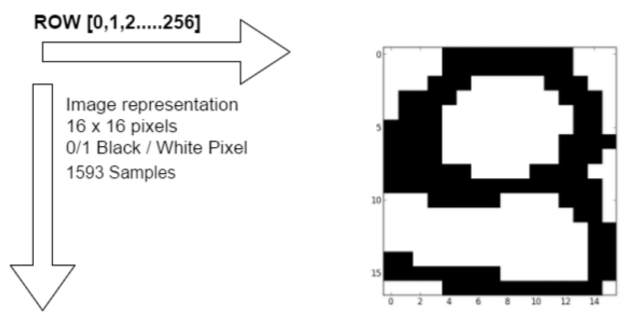
\includegraphics[width=0.8\textwidth]{dataset}
\centering
\caption{Data and Image Representation}
\label{fig:1}
\end{figure}
\begin{figure}[H]
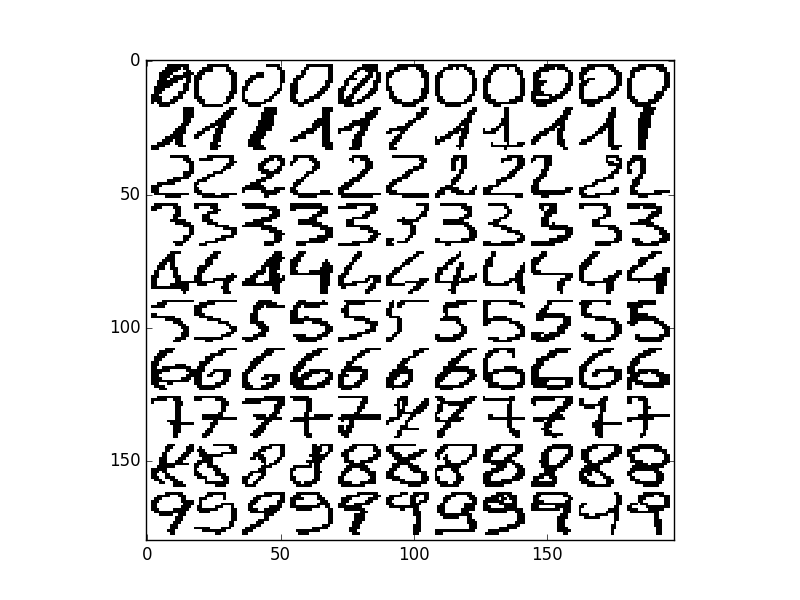
\includegraphics[width=0.5\textwidth]{dataset100}
\centering
\caption{100 digits sample from dataset}
\label{fig:1.1}
\end{figure}
\section{Methods and Experiments}

\subsection{Pre-processing}

It is known that real world data is generally incomplete and full of inconsistent values. Techniques like pre-processing are useful in machine learning in order to make the data ‘look’ better before applying a specific predictive algorithm~\cite{bishop2007pattern}. Generally, these methods can be classified in one of the following: data cleaning, data transformation, data reduction, discretization and normalization/regularization~\cite{rajaraman2012mining}.

This work focuses in the data reduction technique as it helps to reduce the number of dimensions of the dataset. Dimensionality reduction was done through the use of PCA (Principal Component Analysis) which focuses in reducing the number of dimensions of the given matrix by finding the direction (principal components) in which the variance is the greatest~\cite{bishop2007pattern}.

Along with the dimensionality reduction, PCA was also used for compression. Each digit can be easily visualized by plotting a 16 x 16 matrix with the given pixels of the dataset. Therefore, the effects of compression can be easily seen after reconstructing the original matrix through the PCA inverse transformation. 
 
\subsection{Methods}

In this section the algorithms which obtained more than 75\% of accuracy are described. A detailed description is given for the algorithm with best performance, Support Vector Machine.

\subsubsection{Support Vector Machine (SVM)}

SVM performs classification by finding the hyperplane that maximizes the margin between two classes. The vectors that define the hyperplane are the support vectors. Given the labelled data (training set), the algorithm outputs an optimal hyperplane which categorizes the new examples.

We can draw a line on a graph of $x1$ vs $x2$ separating the two classes($y = -1\  or +1$) when $D = 2$ and a hyperplane on graphs of $x1, x2 ...xD$ for when $D > 2$.  This hyperplane can be described by:
\begin{equation}
w \cdot x + b = 0
\end{equation}

where $w$ is normal to the hyperplane and $b/\|w\|$ is the perpendicular distance from the hyperplane to the origin.

Support vectors are the training examples that are closest to the hyperplane and the aim of SVM is to orientate this hyperplane to make it as far as possible from the closest members of both classes.

\begin{figure}[H]
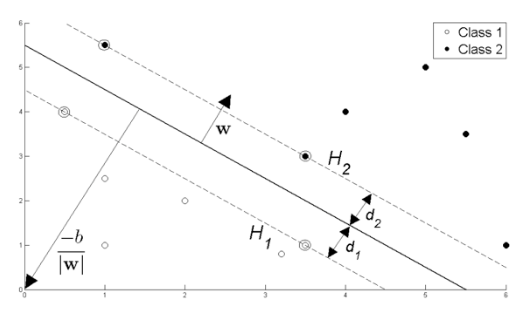
\includegraphics[width=0.6\textwidth]{svm}
\centering
\caption{Hyperplane through two linearly separable classes}
\label{fig:2}
\end{figure}

Referring to Figure~\ref{fig:2}, select $w$ and $b$ such that the training data can be described by:

\begin{equation}
x_i \cdot w + b \geq  +1 \quad for\ y_i = +1
\end{equation}
\begin{equation}
x_i \cdot w + b \leq -1 \quad for\ y_i = -1
\end{equation}

These equations can be combined into:
\begin{equation}
y_i (x_i \cdot w + b) - 1 \geq 0 \quad \forall i
\end{equation}
For the points on the boundary (H1 and H2 in \ref{fig:2}), it can be written as follows:
\begin{equation}
x_i \cdot w + b = +1\ or\ -1  
\end{equation}

In order to orientate the hyperplane to be far from support vectors (maximize margin), the margin $1/\|w\|$   should be maximised. This is equivalent to minimising $\|w\|$ or $\frac{1}{2}\|w\|^{2}$:
\begin{gather}
min \frac{1}{2} \|w\|^{2} \\ 
s.t\  y_i (x_i \cdot w + b) -1 \geq 0 \quad \forall i
\end{gather}

In order to cater for the constraints in this minimization, we need to allocate them Lagrange multipliers $\alpha$, where $\alpha_{i} \geq 0 \forall i$:
\begin{equation}
L_P \equiv \frac{1}{2} \|w\|^{2} - \sum^{L}_{i=1}  \alpha_{i}y_i (x_i \cdot w + b) + \sum^{L}_{i=1} \alpha_{i}
\end{equation}

This minimization can be done by finding $w$ and b which minimizes, and the $\alpha$ which maximizes the above equation. This can be done by differentiating $L_P$ with respect to  w and b and setting the derivatives to 0. By doing that:
\begin{gather}
L_D \equiv \sum^{L}_{i=1} \alpha_{i} - \frac{1}{2} \sum_{i,j} \alpha_{i}\alpha_{j}y_i y_j x_i x_j \quad s.t.\ \alpha_{i} \geq 0 \quad \forall i \\
\sum^{L}_{i=1}  \alpha_{i}y_i = 0  
\end{gather}

Having moved from minimizing $L_p$ to maximizing $L_D$, $w$ and $b$ can be calculated and each new data point can be classified. This new formulation $L_D$ is referred to as the Dual form of the Primary $L_P$. The Dual form requires only the dot product of each input vector $x_i$ to be calculated, this is important for the Kernel Trick~\cite{fletcher2009support}.
\paragraph{Kernel Support Vector Machines}
The original SVM optimal hyperplane algorithm is a linear classifier. Kernel SVM is used to handle data which are not fully linearly separable. The basic idea is to gain linear separation by mapping the data to a higher dimensional space. $k(x_i, x_j)$ is an example of a family of functions called Kernel Functions. Kernel functions are basically based on the inner products of two vectors. This means that if the functions can be recast into a higher dimensionality space by some potentially non-linear feature mapping function $x \rightarrow \varphi(x)$, only inner products of the mapped inputs in the feature space need be determined without us needing to explicitly calculate $\varphi$.

\subparagraph{Polynomial kernel}
\begin{equation}
k(x, z) = (1 + x^T z)^2
\end{equation}

\subparagraph{Gaussian Kernel}
\begin{equation}
k(x, z) = exp(-\gamma\|x-z\|^2)
\end{equation}

The library scikit-learn has an implementation of SVM using \lstinline|sklearn.svm|. For the svm classifier, the important  parameters used are 1) parameter \lstinline|C|, which trades off the misclassification of training examples against simplicity of the decision surface. It is common for all kernel functions. A low \lstinline|C| makes the decision surface smooth, while a high \lstinline|C| aims at classifying all training examples correctly 2) parameter \lstinline|gamma| defines how much influence a single training example has. The larger the \lstinline|gamma| is, the closer other examples must be to be affected 3) parameter \lstinline|Kernel| takes in the type of kernel function used for classification. The values can be linear, polynomial, sigmoid or rbf~\cite{svmsklearn}.


\subsubsection{Random Forest}
Random forest can be explained as a large collection of de-correlated trees. Trees can be used as a predictive model which maps observations about an item to conclusions about the item's target value. One drawback of this model are its propensity  to overfit to the data. To avoid this issue random forest algorithm builds several random trees with a specific splitting process. Then, for a regression problem the resulting values of the trees are averaged to get the final predictions, and for a classification problem the most frequent predicted class by the trees is chosen as the final prediction~\cite{friedman2001elements}. 

As the problem under study is a classification task a random forest classifier was used. The scikit-learn library includes a class which implements random forest classifier, \lstinline|sklearn.ensemble.RandomForestClassifier|. To create a \lstinline|RandomForestClassifier| object the most important parameters to be defined are 1)  number of estimators or trees (\lstinline|n_estimators|), 2) maximum depth of the trees from root to the leaves (\lstinline|max_depth|), and  3) the number of features to consider when looking for the best split (\lstinline|max_features|)~\cite{scikit-learn}. 

\subsubsection{Logistic Regression}
Logistic regression sometimes called the logistic model or logit model, analyzes the relationship between multiple independent variables and a categorical dependent variable, and estimates the probability of occurrence of an event by fitting data to a logistic curve. This algorithm uses a sigmoid function, which maps the whole real line to [0,1], which is necessary for the output to be interpreted as a probability. To prevent overfitting, regularization can be used to avoid the parameters of the model reach high values and do not allow generalization~\cite{park2013introduction}.

The scikit-learn library includes an implementation of logistic regression in the class \lstinline|sklearn.linear_model.LogisticRegression|. To create a \lstinline|LogisticRegression| object the main parameter to be passed is 1) \lstinline|C|, which is the inversed regularization strength (the higher \lstinline|C| the less regularization is applied)~\cite{scikit-learn}. 

\subsubsection{K-Nearest Neighbour (KNN)}
Neighbors-based classification is a type of instance-based learning or non-generalizing learning: it does not attempt to construct a general internal model, but simply stores instances of the training data. Classification is computed from a simple majority vote of the nearest neighbors of each point: a query point is assigned the data class which has the most representatives within the nearest neighbors of the point~\cite{knnsklearn}. In k-nearest neighbor learning, the number of samples is specified by the user.

The scikit-learn library implements K nearest neighbor algorithm using \lstinline|sklearn.neighbors.KNeighborsClassifier|. There are 3 important parameters used in this implementation 1) parameter \lstinline|n_neighbors| represents the Number of neighbors  2) parameter \lstinline|p|, an integer, represents the Power parameter for the Minkowski metric and 3) parameter \lstinline|algorithm| takes the values auto, ball\_tree, kd-tree, brute. It actually represents the choice of neighbors search algorithm. When the value is auto, the algorithm decides the best approach for training data~\cite{scikit-learn}.

\subsubsection{Linear Discriminant Analysis (LDA)}
Linear discriminant analysis is a classifier with a linear decision surface. It is an attractive classifier because it provides closed-form solutions that can be easily computed and its proven well in practice.It is inherently multiclass and has no hyperparameters to use. LDA can be used to perform supervised dimensionality reduction, by projecting the input data to a linear subspace consisting of the directions which maximize the separation between classes~\cite{ldasklearn}.

Linear Discriminant Analysis can be implemented by scikit-learn library using \lstinline|sklearn.discriminant_analysis.LinearDiscriminantAnalysis|. The parameter \lstinline|solver| decides if Singular value Decomposition(svd), Least squares solution(lsqr) or Eigenvalue decomposition(eigen) to be used by the algorithm in the classification task. Another parameter is \lstinline|n_components| which represents the number of components for dimensionality reduction~\cite{scikit-learn}.

\subsubsection{Multinomial Naive Bayes}
Naive Bayes algorithms assume the independence of features and apply the Bayes’ theorem for classification. Generally, NB classifiers require a small set of training data to estimate the parameters necessary for classification and they are quite fast in execution. Multinomial NB is a Naive Bayes algorithm for multinomially distributed data.

The scikit-learn library used for the implementation of Multinomial Naive Bayes classifier is \lstinline|sklearn.naive_bayes.MultinomialNB|. The most important parameter used by this classifier is \lstinline|alpha|, which is the smoothing parameter. The smoothing is a way of regularization and it accounts for the features not present in the learning samples and prevents zero probabilities in further computations~\cite{scikit-learn}.

\subsubsection{Gaussian Naive Bayes}
This is another Naive Bayes classifier and it implements the Gaussian Naive Bayes algorithm for classification. The likelihood of the features is assumed to be Gaussian. The scikit-learn library used for the implementation of Gaussian Naive Bayes classifier is \lstinline|sklearn.naive_bayes.GaussianNB|. No particular parameters have been tried in the configuration of this algorithm for this experiment~\cite{scikit-learn}.

\subsection{Implementation Details}

\subsubsection{Parameter selection}
As it is mentioned in the algorithm section, several algorithms were tried with several configurations. The Table~\ref{table:1} show all the combinations used and the best parameter configurations according its accuracy for each of them. Just algorithms which obtained more than 75\% are shown.

\begin{table}[H]
\centering
\begin{tabular}{|l|l|c|l|}
\hline
\multicolumn{1}{|c|}{\textbf{Algorithm}} & \multicolumn{1}{c|}{\textbf{Parameters}} & \textbf{Combinations} & \multicolumn{1}{c|}{\textbf{\begin{tabular}[c]{@{}c@{}}Best parameter\\ configuration\end{tabular}}} \\ \hline
\begin{tabular}[c]{@{}l@{}}Support \\ Vector \\Machine \end{tabular} & \begin{tabular}[c]{@{}l@{}}C: 0.1, 1, 10, 100\\ gamma: auto, 0.03, 0.003\\ 			kernel: rbf, linear, poly, sigmoid\end{tabular} & 48 & \begin{tabular}[c]{@{}l@{}}C: 10,\\ 			gamma: 0.03\\ kernel: rbf\end{tabular} \\ \hline
\begin{tabular}[c]{@{}l@{}}Random\\ 			Forest\end{tabular} & \begin{tabular}[c]{@{}l@{}}n\_estimators: 10, 100, 300, 500        \\ 			max\_features: auto, sqrt, log2        \\ max\_depth: None, 5\end{tabular} & 24 & \begin{tabular}[c]{@{}l@{}}n\_estimators: 300\\ max\_features: log2\\ max\_depth: None\end{tabular} \\ \hline
\begin{tabular}[c]{@{}l@{}}Logistic\\ 			Regression\end{tabular} & C: 0.1, 1, 10, 100 & 4 & C:0.1 \\ \hline
\begin{tabular}[c]{@{}l@{}}K-Nearest\\ 			Neighbour\end{tabular} & \begin{tabular}[c]{@{}l@{}}n\_neighbors: 3, 5, 7        \\ p: 1, 2, 3\\ algorithm: auto, ball\_tree, kd\_tree, brute\end{tabular} & 36 & \begin{tabular}[c]{@{}l@{}}n\_neighbors: 7        \\ p: 3\\ algorithm: brute\end{tabular} \\ \hline
\begin{tabular}[c]{@{}l@{}}Linear 			Discriminant \\ Analysis\end{tabular} & \begin{tabular}[c]{@{}l@{}}solver: svd, lsqr, eigen\\ 			n\_components:3, 5, 8\end{tabular} & 9 & \begin{tabular}[c]{@{}l@{}}solver: eigen\\ n\_components:8\end{tabular} \\ \hline
\begin{tabular}[c]{@{}l@{}}Multinomial\\ 			Naive Bayes\end{tabular} & alpha: 0.1, 0.3, 1 & 3 & alpha: 1 \\ \hline
\begin{tabular}[c]{@{}l@{}}Gaussian\\ 			Naive Bayes\end{tabular} & - & 1 & - \\ \hline
\end{tabular}
\caption{Parameter configurations for algorithms}
\label{table:1}
\end{table}

In addition to the previous parameters, some algorithms accept an optional parameter to make a parallel calculation, such algorithms are Random forest, Logistic regression, and K-nearest neighbors. This behavior can be used just if the parent task running the algorithms is not running in multiprocessing mode.   

\subsubsection{Cross validation}
The main goal of cross-validation is to ensure that every sampling from the original set has the probability of appearing in the training and testing set. The k-fold cross validation strategy is that where the original sample is randomly partitioned into k subsamples and one is left out each iteration~\cite{kohavi1995study}. In the cross validation evaluation procedure experimented in the classifier, 10\% of the given training dataset is taken as test data, the remaining 90\% data (which is considered as the training data in that trial) has been used by the classifier to predict the classes of the test data and this procedure is repeated 10 (k=10) times. 

For this assignment, in every experiment a 10-fold cross-validation procedure was applied. The library scikit-learn implements this process with its class \lstinline|sklearn.cross_validation| which includes the function \lstinline|cross_val_score| that calculates a score specified by the user using cross-validation~\cite{scikit-learn}.


\subsubsection{Multiprocessing and Profiling}
In order to speed up the task which run all the algorithms a multiprocessing procedure was implemented and a profile of the task with and without multiprocessing was done. To implement the multiprocessing procedure the Python library joblib was used and for profiling the algorithms the package cProfile was used.

The results of applying multiprocessing are considerable. According to the profile without applying multiprocessing, run all the algorithms it takes 470.9 seconds with 80,692,163 function calls. The same process but implementing multiprocessing takes 151.2 seconds with 104,841 function calls. 

\subsubsection{Hardware and Software Specifications}

The computer where the experiments were run has the next specifications: Intel i7-6700k 8 cores 4.2Ghz 16GB RAM 512 GB SSD.

The development of the project was done in the software tool PyCharm using Python 3.5.

\subsection{Experiments}
As machine learning has a broad spectrum of different algorithms, it is required to thoroughly test  the highest number of possible combinations in order to achieve optimal results. This work was focused in testing 9 popular algorithms: SVM, Random Forest, Logistic Regression, KNN, Linear Discriminant Analysis, Multinomial Naive Bayes, Gaussian Naive Bayes, AdaBoost, and Decision Trees. In total, there were 169 different combinations of algorithms/configuration and from these we took the top 2 algorithms. Table~\ref{table:2} shows the best result of each algorithm. As all classes have a similar number of instances, accuracy was used as a metric of comparison. 

\begin{table}[H]
\centering
\begin{tabular}{|l|c|l|}
\hline
\multicolumn{1}{|c|}{\textbf{Algorithm}} & \textbf{Accuracy} & \multicolumn{1}{c|}{\textbf{Parameters}}          \\ \hline
Support Vector Machine                                      & 95.92\%           & C=10, gamma=0.03, kernel= rbf                     \\ \hline
Random Forest                             & 94.96\%           & n\_estimators=300, max\_features=log2, max\_depth=None \\ \hline
Logistic Regression                      & 91.58\%           & C=0.1, multi\_class=ovr                           \\ \hline
K-Nearest Neighbors                               & 90.82\%           & n\_neighbors=7, p=3, algorithm=brute                    \\ \hline
Linear Discriminant Analysis             & 88.65\%           & solver=eigen, n\_components=8                      \\ \hline
Multinomial Naïve Bayes                  & 84.58\%           & alpha=1                                           \\ \hline
Gaussian Naïve Bayes                     & 79.21\%           &                                                   \\ \hline
AdaBoost                                 & 71.68\%           & n\_estimators=10, learning\_rate=0.3                  \\ \hline
Decision Trees                           & 70.34\%           & max\_depth=None, max\_features=sqrt               \\ \hline
\end{tabular}
\caption{Best results for each algorithm}
\label{table:2}
\end{table}

As it can be seen, Support Vector Machines and Random Forest were the best algorithms for this task. A thorough discussion will be given along with a personal reflection on why these two algorithms performed the best in the next sections.

\subsubsection{PCA for Data Compression and Dimensionality Reduction}

Matrix decomposition is an useful way of reducing the amount of processing and memory needed by a computer to process matrices where the number of features (columns) are very big~\cite{rajaraman2012mining}. However, when using images, decomposition for data compression can also be easily identified by the reduction in the overall ‘quality’ of the picture. Figure~\ref{fig:3}, shows the digits representations of 3 different explained variances of PCA. For both 90\% and 50\% explained variance, it can be seen that the digits are still recognizable, which can be supported by the 96\% and 93\% accuracy obtained through applying our predictive algorithms in the reduced dataset. Still supporting this conclusion, it can be noted that with only 10\% of the explained variance, the numbers are barely recognizable, and, as a result, yielded a poor accuracy (49\%).

\begin{figure}[H]
\includegraphics[width=\textwidth]{pca_all}
\centering
\caption{Resutls applying PCA and reconstruction of images using different  explained variances}
\label{fig:3}
\end{figure}

%Figure XX: PCA used for Compression and Dimensionality Reduction


\subsection{Comparison with MNIST}

Over the last year many competitions in handwritten digit recognition have been held in the MNIST (Mixed National Institute of Standards and Technology database). This dataset contains 60,000 examples of training set and 10,000 examples of test set. In 2002, DeCoste and Scholkopf reached 99.44\% accuracy rate when they applied virtual SVM algorithm (deg-9 poly, 2-pixel jittered)~\cite{decoste2002training}. In their research, the handwritten images were positioned in a 28 x 28 features (pixels) for classification. Their features were gray scale pixels ranging from 0 to 255.

Comparing to their high resolution ratio, this work uses 16 x 16 features (pixels), and assigned only boolean value (0/1) to the field. In order to reach higher accuracy, there are few things that can be improved in this experiment. First, increase the size of features that contains the handwritten image, for instance, using 28 x 28 images. Second, apply gray scale range instead of boolean features which can give more information for each feature. Third, optimize the algorithm to fit the problem itself trying more options for tuning and testing. Finally, another factor that can influence the accuracy level is the size of the data set. The current dataset contains only 1,593 instances which is really small compared to MNIST. A bigger dataset should improve the accuracy of the classification task.

\section{Discussion}

SVM is a supervised learning model that analyses data and is a suitable option for recognizing patterns. Some of the best characteristics of SVM are 1) memory efficiency - as it uses only a subset of training points called support vectors  in the decision function 2) Versatility - different Kernel functions can be specified for the decision function. Recent researches show that SVM demonstrated its accuracy, space efficiency and time efficiency in handwritten digit recognition~\cite{kouropteva2003classification}. Many improvements by combining SVM with other algorithms  were conducted to increase its accuracy~\cite{keysers2007comparison}. In 1998, B. Scholkopf etc. applied virtual SVM on handwritten digit recognization, it reached 99.20\% accuracy rate~\cite{scholkopf1998prior}. In 2002, D. DeCoste and B. Scholkopf. used virtual SVM (jitter) to get 99.37\% accuracy rate~\cite{decoste2002training}. In our experiment also, SVM outperformed other algorithms in terms of accuracy for the chosen dataset. Therefore, SVM is selected as the  the main topic of discussion in this report.

Although SVM has all the aforementioned advantages, it is worth to note its caveats as there is still place for improvement in the handwriting recognition field of study. In 2009, Marthias M proposed an alternative implementation of the popular SVM algorithm. In his studies, Marthias states that “SVM classifiers, like other kernel machines, gives a poor generalization when the hyperparameters are not tuned efficiently”. Thus, his work proposed a model selection technique for SVM using empirical error criterion through the LOO cross-validation procedure. LOO is the special case of cross-validation where the number K of folds is equal to the training set size. All the tests were also applied in the MNIST database, and the algorithm achieved higher performance when compared to the traditional SVM model~\cite{adankon2009model}.

On the other hand, Random Forest is still an extremely efficient and popular algorithm nowadays. The algorithm presents a straightforward implementation, a reasonable computing cost and a very good performance in terms of classification accuracy. However, in all the tests it was still outperformed by SVM. Studies like Bernand S, 2009 reveals good variants of the Random Forest algorithm in the MNIST database but they still reach poor accuracy when compared to the SVM results~\cite{bernard2007using}.

This study leads us to believe that SVM presents one of the best models for Handwritten recognition. Working on model selection and kernel parameters tuning is a good start for improving results even further.

\section{Conclusions and future work}

The development of this work has proved that machine learning can be a powerful tool in the handwriting recognition field. Even though the dataset used in this paper had limited features and a low amount of samples, it is believed that the results are already satisfactory for this problem. A good example of how a better dataset can help to improve the results is provided by the MNIST (Mixed National Institute of Standards and Technology database) work as their accuracy was close to 100\%. Given more research time it could be possible to improve the accuracy by performing some feature engineering in the dataset along with more experiments with predictive algorithms. 

Some possible future work could be to include recent techniques that have shown remarkable results in MNIST competitions. For example, deep learning techniques are the state of the art in this kind of problems reaching a test rate error of 0.21\% (99.79\% of accuracy) by Li Wan et al. using a Convolutional Neural Networks with DropConnect methodology in 2013~\cite{wan2013regularization}. However, to reach these results the amount of data need to be bigger than what actually the chosen dataset has, but still it will be possible to improve the results shown in this report.

All in all, this work not only provided very good insights in how to use machine learning techniques but also helped the understanding of the concepts taught during the Knowledge Discovery subject.

\nocite{nbsklearn}

%biblio
\bibliographystyle{unsrt}
\bibliography{biblio}

\section{Appendix}

\subsection{Instructions}
The instructions of how to run the code are inside the README.md file.

\subsection{Links to external open-source libraries used for analyses}
\begin{itemize}
\item Semeion Repository - \url{https://archive.ics.uci.edu/ml/datasets/Semeion+Handwritten+Digit}
\item Python - \url{https://www.python.org/}
\item scikit-learn - \url{http://scikit-learn.org/}
\item Pandas - \url{http://pandas.pydata.org/}
\item matplotlib - \url{http://matplotlib.org/}
\item joblib - \url{https://pythonhosted.org/joblib/}
\item cProfile - \url{https://docs.python.org/3.5/library/profile.html}
\end{itemize}



\end{document}
